\section{零假设下的有限样本校准结果}\label{sec:h0}

本节报告 28 个唯一零假设配置下，朴素置换（M0）与依赖乘子自助法（M1）的有限样本 I 类错误率。分析重点为条件化校准表面及其逐格边界，汇总均值仅作为辅助描述。

\subsection{双预算制度下的校准表面}\label{sec:h0-heatmap}

图~\ref{fig:m0-surface} 给出 M0 在两种预算制度下的 I 类错误率表面，图~\ref{fig:m1-deviation} 给出 M1 的校准偏差 $\widehat\alpha-0.05$。两幅图均含固定窗口数与固定观测长度两个面板，纵轴保留数据生成过程、$\rho$ 与步长三个条件维度。两图共有 16 个“条件--表示--方法”数值因共享几何 $s=16$、$T=3120$、$M=192$ 而被有意重复展示，用于分别解释两种预算制度，不应视为两份独立证据。完整 $16\times4$ 热图见补充材料。

\begin{figure}[ht]
\centering
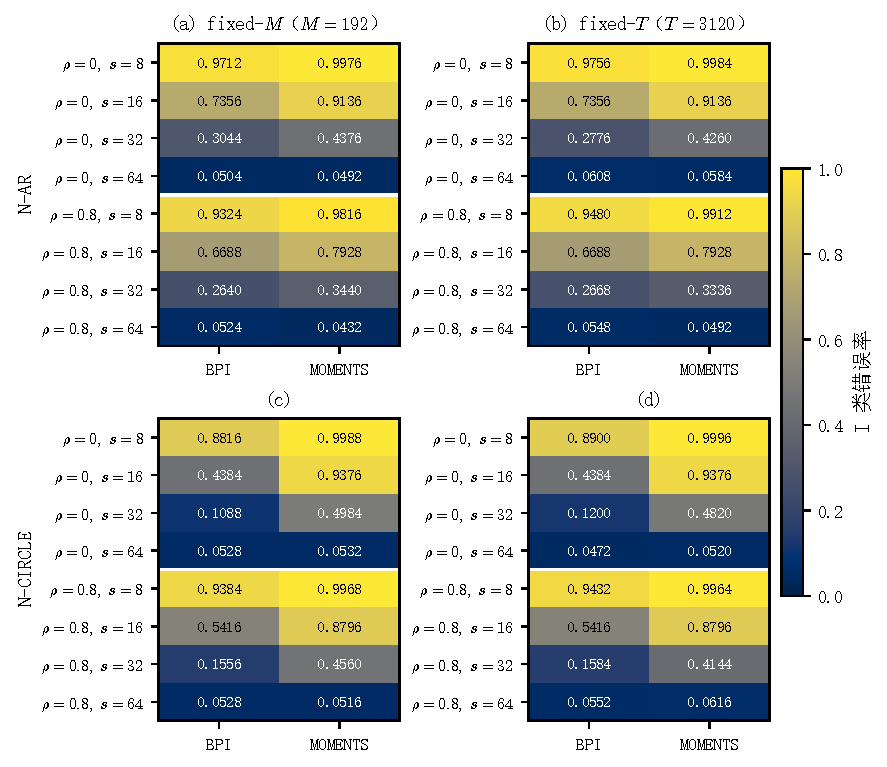
\includegraphics[width=0.92\textwidth]{../artifacts/figures/Figure3_M0_type1_surface.pdf}
\caption{M0（朴素置换）在两种预算制度下的有限样本 I 类错误率表面。左：固定窗口数（$M=192$）；右：固定观测长度（$T=3120$）。色标 $[0,1]$，格内标注三位小数拒绝率。}\label{fig:m0-surface}
\end{figure}

\begin{figure}[ht]
\centering
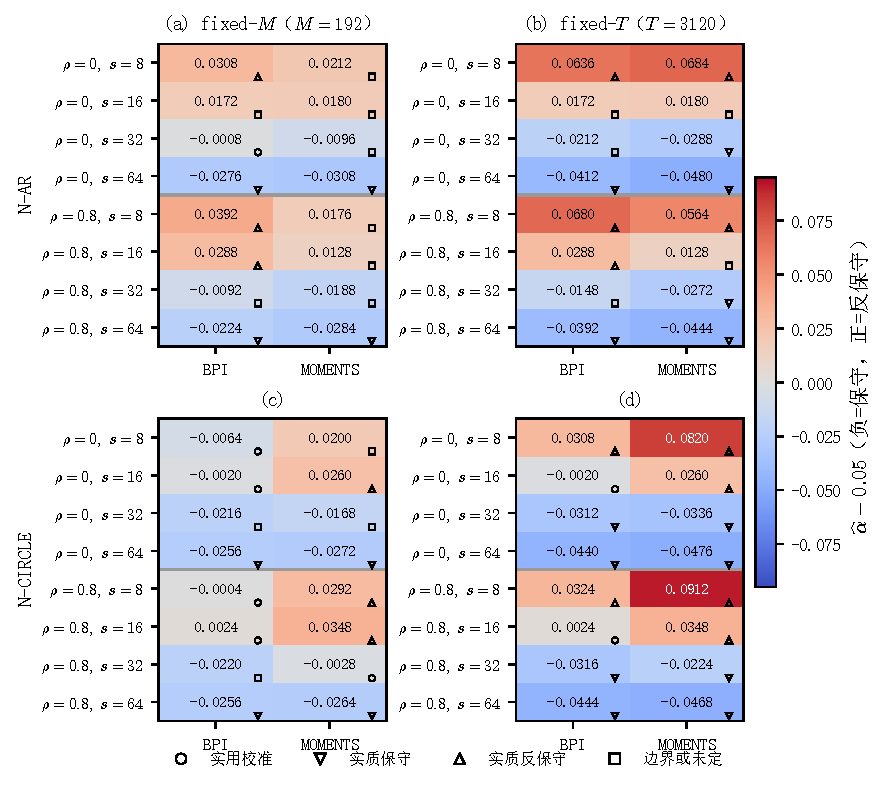
\includegraphics[width=0.92\textwidth]{../artifacts/figures/Figure4_M1_deviation_surface.pdf}
\caption{M1（依赖乘子法）在两种预算制度下的校准偏差 $\widehat\alpha-0.05$。负值表示保守，正值表示反保守，0 对应名义水平 $0.05$。符号编码逐格 Wilson 判定：圆圈=实用校准，下三角=实质保守，上三角=实质反保守，方块=边界或不确定。}\label{fig:m1-deviation}
\end{figure}

M0 的校准表现对窗口重叠高度敏感。BPI/M0 的逐格拒绝率介于 $0.0472$ 和 $0.9756$ 之间，MOMENTS/M0 介于 $0.0432$ 和 $0.9996$ 之间；在多数重叠配置中，两者均远高于名义水平。M1 明显压缩了极端反保守性，其对应范围分别为 $0.0056$--$0.1180$ 和 $0.0020$--$0.1412$。然而，M1 的拒绝率同时分布在名义水平以下和以上，表明依赖感知乘子改变了校准表面的形态，却未在所有有限样本配置中实现统一校准。

上述范围也说明，单一总体平均会掩盖具有相反方向的局部偏差。某些配置中的保守性和另一些配置中的反保守性可以在汇总后相互抵消，因此本文以逐格有效尺寸作为主要报告单位。

\subsection{逐格校准分类}\label{sec:h0-classify}

共有
\[
 28\text{（零假设配置）}\times2\text{（表示）}\times2\text{（方法）}=112
\]
个逐格评价单元。依据第~\ref{sec:estimands} 节的预设规则，表~\ref{tab:calibration}汇总四类校准状态。

\begin{table}[ht]
\centering
\caption{逐格校准分类计数（每行 $n=28$）。完整 112 行拒绝率、Wilson 区间与分类结果见补充材料。}\label{tab:calibration}
\begin{tabular}{llcccc}
\toprule
表示 & 方法 & 实用校准 $n\,(\%)$ & 实质保守 $n\,(\%)$ & 实质反保守 $n\,(\%)$ & 边界/未定 $n\,(\%)$\\
\midrule
BPI & M0 & 7 (25.0) & 0 (0.0) & 20 (71.4) & 1 (3.6)\\
BPI & M1 & 5 (17.9) & 10 (35.7) & 7 (25.0) & 6 (21.4)\\
MOMENTS & M0 & 6 (21.4) & 0 (0.0) & 20 (71.4) & 2 (7.1)\\
MOMENTS & M1 & 1 (3.6) & 12 (42.9) & 7 (25.0) & 8 (28.6)\\
\bottomrule
\end{tabular}

\begin{minipage}{0.94\textwidth}
\vspace{0.4em}
\footnotesize 注：实用校准采用 90\% Wilson 区间完整落在等效带 $[0.035,0.065]$ 内，对应预设的实用等效性判据（两个单侧 5\% 判定等价于一个 90\% 双侧区间）；实质保守要求 95\% 区间完整位于实用带下方，实质反保守要求 95\% 区间完整位于实用带上方；边界/未定为既不满足实用校准、也不满足实质保守或实质反保守的剩余状态。上述计数为预设设计网格内的描述性分布，不构成方法在更广参数空间中的通过率。
\end{minipage}
\end{table}

对两种表示，M0 均有 $20/28$ 个配置被判为实质反保守，且没有配置被判为实质保守。M1 的分类则分散于实用校准、实质保守、实质反保守和边界未定四类：BPI/M1 中四类计数依次为 $5$、$10$、$7$ 和 $6$，MOMENTS/M1 中依次为 $1$、$12$、$7$ 和 $8$。这些计数描述预设设计网格内的有限样本分布，不应解释为方法在更广参数空间中的“通过率”。

\subsection{主对比 P1--P3}\label{sec:h0-primary}

表~\ref{tab:primary}报告三个预先冻结主对比的点估计、边际 95\% basic 自助区间和 Holm 校正结果。按照第~\ref{sec:primary} 节的单侧阈值与多重性规则，三项对比均满足预设支持标准。

\begin{table}[ht]
\centering
\caption{主对比 P1--P3 的效应量与推断结果。置信区间为边际 95\% basic 自助区间；Holm 校正 $p$ 由 10,000 次配对 cluster bootstrap 的尾部计数按加一规则计算（$p=(1+\#\{\text{尾部}\})/10001$）。}\label{tab:primary}
\begin{tabular}{llccccc}
\toprule
对比 & 估计量方向 & 点估计 & 预设阈值 & 超额效应 & 95\% basic CI & Holm $p$\\
\midrule
P1（固定 $M$ 重叠） & $s{=}16$ 减 $s{=}64$ 的 M0 拒绝率差 & 0.5354 & 0.10 & 0.4354 & $[0.5210,0.5494]$ & 0.00030\\
P2（固定 $T$ 步长） & $s{=}16$ 减 $s{=}64$ 的 M0 拒绝率差 & 0.5330 & 0.10 & 0.4330 & $[0.5194,0.5462]$ & 0.00030\\
P3（M1 非重叠保守性） & $0.05$ 减 M1 拒绝率 & 0.0266 & 0.01 & 0.0166 & $[0.0224,0.0308]$ & 0.00030\\
\bottomrule
\end{tabular}

\begin{minipage}{0.94\textwidth}
\vspace{0.4em}
\footnotesize 注：三项尾部计数经真实 bootstrap 抽样核验均为 0，故原始 $p=1/10001\approx9.999\times10^{-5}$；经 Holm 逐步校正后三项调整 $p$ 均为 $3/10001\approx0.00030$。点估计与阈值之差为超额效应；正文按预设单侧阈值与多重性规则给出支持与否的表述，表中仅列统计量。
\end{minipage}
\end{table}

在固定窗口数制度下，$s=16$ 相对于 $s=64$ 的 M0 拒绝率差异，经两个数据生成过程等权平均后为 $0.5354$；在固定观测长度制度下，相应差异为 $0.5330$。两项区间的下界均远高于预设阈值 $0.10$，相对于该阈值的超额分别为 $0.4354$ 和 $0.4330$。因此，在两个预设数据生成过程、$\rho=0$ 和 BPI 表示的等权平均意义下，重叠相关的严重失校准在两种预算制度中均稳定出现。该结论不延伸为每一数据生成过程、每一依赖水平或每一表示下的必然规律。

P3 的估计为 $0.0266$，其 95\% 区间完整高于预设阈值 $0.01$。这表明在 $\rho=0$、$s=W=64$、固定 $M=192$ 的非重叠端，当前 M1 带宽规则产生了可检测的保守偏差。该结果同时提示，依赖感知校准器在窗口不重叠时也需要接受有限样本验证。

\subsection{原序列依赖的效应修饰}\label{sec:h0-rho}

为避免将单一步长下的 $\rho$ 差异与重叠效应修饰混为一谈，次级分析采用步长对比的差。对数据生成过程 $g$、表示 $\varphi$ 和预算制度 $r$，定义
\begin{align}
 D_{g,\varphi}^{(r)}(\rho)
 &=\pi_{g,\rho,16,\mathrm{M0},\varphi}^{(r)}
  -\pi_{g,\rho,64,\mathrm{M0},\varphi}^{(r)},\\
 I_{g,\varphi}^{(r)}
 &=D_{g,\varphi}^{(r)}(0.8)-D_{g,\varphi}^{(r)}(0).
 \label{eq:rho-interaction}
\end{align}
其中 $I_{g,\varphi}^{(r)}$ 衡量原序列依赖对“$s=16$ 相对于 $s=64$”拒绝率差异的修饰。

描述性估计显示，BPI/N-AR 的 $I^{(M)}$ 和 $I^{(T)}$ 分别为 $-0.0688$ 和 $-0.0608$，BPI/N-CIRCLE 分别为 $0.1032$ 和 $0.0952$；MOMENTS/N-AR 分别为 $-0.1148$ 和 $-0.1116$，MOMENTS/N-CIRCLE 分别为 $-0.0564$ 和 $-0.0676$。修饰方向随数据生成过程和表示而变化：正值表示 $\rho=0.8$ 放大步长对比，负值表示其缩小步长对比。由于该分析为次级描述，且不同条件的符号并不一致，本文不据此提出原序列依赖具有统一单调作用的结论。
